\documentclass[11pt, a4paper]{article}
\usepackage[a4paper, total={6in, 9.5in}]{geometry}

\title{\textbf{\Huge Gravitational Wave Physics and LIGO}}

\usepackage{amsmath, tensor, gensymb, graphicx, hyperref, authblk, amsfonts, amssymb, verbatim, wrapfig, subfig}
\usepackage[T1]{fontenc}
\usepackage[utf8]{inputenc}
\usepackage[english]{babel}
\usepackage[bottom]{footmisc}
\usepackage[sorting = none]{biblatex}

\hypersetup{
    colorlinks=true,
    linkcolor=blue,
    urlcolor=blue,
    citecolor=black}
\urlstyle{same}

\addbibresource{bibliography.bib}

\author[1]{Sagar JC}
\author[1]{Aditya Srivatsa}
\author[1]{Ajith U Shanbhag}
\author[2]{Kushal J}
\author[3]{Hardik Medhi}
\author[4]{Bhavya Goradia}
\author[5]{Kshitija Kshirsagar}
\author[6]{Tasmi Memon}
\author[7]{Samrudhi R Kanjarpane}
\author[8]{Ajay Atwal}
\author[9]{Divyanshi Agrawal}
\author[9]{Kirti Jadhav}
\author[9]{Ved Deshpande}
\author[10]{Dhyan Gandhi}

\affil[1]{St. Joseph's College, Bengaluru}
\affil[2]{Christ Junior College, Bengaluru}
\affil[3]{REVA University, Bengaluru}
\affil[4]{KJ Somaiya College of Engineering, Mumbai}
\affil[5]{Institute of Science, Nagpur}
\affil[6]{Maharaja Sayajirao University, Vadodara}
\affil[7]{Poornaprajna College, Udupi}
\affil[8]{University of Hyderabad, Hyderabad}
\affil[9]{St. Xavier's College, Mumbai}
\affil[10]{Manipal Institute of Technology, Udupi}

\renewcommand\Authands{ and }

\date{\today}

\begin{document}
\maketitle

\section*{Acknowledgement}
\input{Acknowledgement}

\pagebreak
\begin{center}
    \section*{Abstract}
\end{center}

Gravitational waves was first proposed by Albert Einstein in his 1916 paper on "The Theory of General Relativity". Gravitational waves are disruptions or “ripples” of the space time fabric, caused due to the acceleration of massive bodies, such as neutron stars or black holes. These disruptions stretch and squeeze the space as they pass by, and travel at the speed of light from its source in all directions. Before the discovery of gravitational waves, we were limited to looking at the universe only using electromagnetic waves emitted by various celestial objects. We go through one of the results of general relativity which is gravitational waves and explain it's theoretical aspect like linearized theory and experimental setup that provides us with the data that we can use to understand the nature of the sources of these waves and the universe itself. Here we are reviewing some of their work to better understand not only the reasons for their use, but also the very methods in which they are formed and how we can detect them. The paper consist of LIGO, the most prominent Gravitational Wave detector made by mankind yet. We study the various disturbances affecting LIGO, and the causes behind them. The different methods used behind the extraction of signals once the noise has been reduced has been discussed as well. Finally we explain the various observations of LIGO and Advancements of LIGO. 


\providecommand{\keywords}[1]
{
  \small	
  \textbf{\textit{Keywords---}} #1
}

\keywords{General Relativity, Space time, Tensors, indices, Field equations, Wave equation, Polarization, Energy Flux, Doppler effect, Inverse square law, Inspiral mechanism, Black holes, Neutron stars, Pulsars, Revolving Binary system, LIGO, Interference, Coherency, Laser, CMB, Noise isolation, Signal extraction, Template matching}
\pagebreak

\tableofcontents
\pagebreak

\section{Introduction}
\hspace{0.5cm} General relativity is an important part of physics which helps us understand our universe in a large scale like black holes, gravitational waves and our expanding universe. It describes gravity as a property of space and time rather than a force as mentioned by Newton. It tells us that the curvature of space time is related to energy and momentum which is present inside matter. Einstein's feild equations also theorizes various phenomena such as the wrapping of space time and gravitational waves. It helps us to understand the region of space having black holes or neutron stars, or a system of dynamical heavy masses which causes great changes in gravity. We know that there are three dimensions of space which we can interact with. But Einstein included time also as the fourth dimension. Thus space time is four dimensional in nature, consisting of three dimensions of space and one dimension of time. When there is no matter, space time is flat, and the shortest distance between any two points will be a straight line. But in the presence of matter, the shape of space time is altered, making the shortest distance between two points a curved line, which is also known as a `Geodesic'.

\begin{figure}[h]
    \centering
    \includegraphics[scale=0.2]{images.tex/illus_3dspace1.jpg}
    \caption{Curved space-time in presence of mass. Source:- \href{https://www.forbes.com/sites/startswithabang/2019/02/16/ask-ethan-how-can-we-measure-the-curvature-of-gravity/?sh=13c20ec1134f}{Forbes.com}}
\end{figure}

If there are two giant masses orbiting around each other, it results in the formation of ripples in space time which is called as gravitational waves. These ripples move with the speed of light. The farther they move away from their source, the weaker they get. Hence the gravitational waves which are detected are very weak due to various reasons, but are good source of information.\\ 

In 1916, Einstein predicted that two bodies orbiting each other would not be in the same orbit all the time, instead they lose energy and in doing so emit gravitational waves. According to his mathematics he showed that two massive accelerating objects such as neutron stars or black holes, while orbiting each other, generate ripples and disrupt the space time causing waves which propagates in every direction away from the source. These ripples carry information about their origin and about gravity as well. The strongest gravitational waves are generated due to colliding black holes or neutron stars. After half a century, the first indirect proof of gravitational waves was given in the year 1974 when astronomers Jocelyn Bell and Antony Hewish discovered a pulsar which produced a gravitational wave. After this they observed how the stars changed their orbit as the time passes. They observed that the stars were getting closer to each other at the rate which was predicted by Einstein in his General Theory of Relativity by producing gravitational waves.\\ 

On September 14, 2015, LIGO detected a signal which was due to the collision of two massive black holes which occured 1.3 billion years ago. After analyzing the phenomena, it was observed that the wave was caused due to the objects which are 29 and 36 times more massive than the sun, orbiting with a speed of $58.33\,ms^{-1}$ just before they collided. The gravitational waves which were generated near the source were very large but by the time they were detected here on earth, their strength was so small that their effect on the LIGO was 10000 times smaller than a Proton.

\pagebreak



\section{Linearized theory of Gravitational waves}
Linearized theory of Gravitational waves is a basic understanding of gravitational waves based on an assumption that any perturbation in space time can be approximated to a linear factor whose degree is One. This simplifies the calculations a lot. More over since the sources of gravitational waves are very far away, the effects they produce here on earth will be very small. So we can neglect the higher degree of perturbation and linearize it to the first degree. \\

Einstein's field equations are a set of ten tensor equations which describe gravity as a curvature in space time. Below equation is one among them: 
\begin{equation}
    G_{\mu\nu}= \frac{8 \pi  G}{c^{4}}  T_{\mu\nu}
\end{equation}
This is a tensor equation which describes gravity in terms of Einstein's tensor, $G_{\mu\nu}$ which is directly dependent on the geometry of space-time which is altered by the stress-energy tensor $T_{\mu\nu}$. Another field equation that relates the geometry or curvature of space-time to stress-energy tensor is 

\begin{equation}
    R_{\mu\nu}-\frac{1}{2}g_{\mu\nu}R=\frac{8\pi G}{c^{4}}T_{\mu\nu}
\end{equation}
where $R_{\mu\nu}$ is the Riemann tensor which describes the curvature of space-time, $R$ is the scalar curvature and $g_{\mu\nu}$ is the gravitational field tensor. Any change in matter distribution will be recorded in in $T_{\mu\nu}$. So if $T_{\mu\nu}$ changes then according to equation 2, gravitational field tensor $g_{\mu\nu}$ also has to change. If $h_{\mu\nu}$ is the perturbation induced in space-time then the new gravitational field tensor $\tilde{g}_{\mu\nu}$ is given by \cite{Kokkotas_2008}

\begin{equation}
    \tilde{g}_{\mu\nu} = g_{\mu\nu} + h_{\mu\nu}
\end{equation}

\noindent To get the new gravitational field, the field equation should be solved for $\tilde{g}_{\mu\nu}$ which gives 

\begin{equation}
    \tilde{h}_{\mu\nu} = h_{\mu\nu} - \frac{1}{2} \, \eta_{\mu\nu} \, h^{\alpha}_{\alpha}
\end{equation}
 where $\eta_{\mu\nu}$ is the gravity where space is flat i.e. $\eta_{\mu\nu} = g_{\mu\nu}$ and $h^{\alpha}_{\alpha}$ is summed for all spatial coordinates i.e. $\alpha$ takes values $(1,2,3) $ which corresponds to $(x,y,z)$. The admitted solutions for this variations in space time $\tilde{h}_{\mu\nu}$ has solution in the form of 
 
 \begin{equation}
     \tilde{h}_{\mu\nu} = A^{\mu\nu}\, e^{ik_{\alpha}x^{\alpha}}
 \end{equation}
 
 \noindent This is a 3D wave equation where $A^{\mu\nu}$ is the Amplitude tensor, $i = \sqrt{-1} $, $k_{\alpha} = (k_{x},k_{y},k_{z})$ is the wave vector and $x^{\alpha} = (x^{1},x^{2},x^{2}) = (x,y,z)$ is the position vector.
 \\
 
 Thus we can say that whenever a body causes disturbances in the curvature of space-time, these disturbances travel through space in the form of waves whose speed is equal to the speed of light.  
 
\begin{figure}[h]
     \centering
     \includegraphics[scale=0.145]{images.tex/gw_representation.png}
     \caption{A computer simulated 3D Gravitational wave. Source:- \href{https://www.universetoday.com/127255/gravitational-waves-101/}{Universetoday.com}}
 \end{figure}

\pagebreak


\section{Properties of Gravitational waves}
In this section we shall know about the properties of gravitational waves. Gravitational waves can be characterised by its frequency, amplitude and period. They propagate with the same speed as that of electromagnetic waves. Unlike Electromagnetic waves, the wavelength of GW’s can range from a kilometer to the size of the universe itself. Since the wavelength of gravitational waves is larger than the source, they cannot be used for imaging. In contrast to electromagnetic waves which are polarised at 90 degree, i.e orthogonal plane polarized EM waves have their plane 90 degrees apart, where as for polarized gravitational waves the plane of polarization will be 45 degree apart, which will be discussed in the next session. GWs do not interact with matter, but electromagnetic waves do. Electromagnetic waves are known to exhibit a wave-particle duality nature unlike Gravitational waves, the nature of which is still unknown. Although there are quite a few similarities between these two, gravitational waves open a new different window to view the universe. \cite{Thorne:1995xs}

\begin{figure}[h]
    \centering
    \includegraphics[height= 7cm, width=9cm]{images.tex/GW_propagation.jpg}
    \caption{Propagation of GW wave. Source :- \href{https://www.einstein-online.info/en/spotlights/gravwav/gravwav-sub01/}{Einstein-online.info}}
\end{figure}

\begin{figure}[h]
    \centering
    \includegraphics[height= 8.7cm, width=12cm]{images.tex/EM_propagation.png}
    \caption{Propagation of EM wave. Source :-\; \href{https://www.toppr.com/guides/physics/communication-systems/propagation-of-electromagnetic-waves/}{Topper.com}}
\end{figure}

\pagebreak

\subsection{Polarization of Gravitational waves}


Gravitational waves can also be polarized. Since they are three dimensional waves their polarization can be restricted to two forms where the the amplitude tensor $A^{\mu\nu}$ has two forms $A^{\mu\nu}_{+}$ and $A^{\mu\nu}_{\times}$ which are orthogonal to each other \cite{Dirkes_2018}. They can be represented as 

\begin{equation}
    A^{\mu\nu}_{+} = h_{+}\, \varepsilon^{\mu\nu}_{+}
\end{equation}

\begin{equation}
    A^{\mu\nu}_{\times} = h_{\times} \,\varepsilon^{\mu\nu}_{\times}
\end{equation}

\noindent where $\varepsilon^{\mu\nu}_{+}$ and $\varepsilon^{\mu\nu}_{\times}$ are unit polarization tensors.

\begin{equation}
\varepsilon^{\mu\nu}_{+} =
\begin{bmatrix}
0 & 0 & 0 & 0 \\
0 & +1 & 0 & 0 \\
0 & 0 & -1 & 0 \\
0 & 0 & 0 & 0 \\
\end{bmatrix}
\end{equation}
\\
\begin{equation}
\varepsilon^{\mu\nu}_{\times} =
\begin{bmatrix}
0 & 0 & 0 & 0 \\
0 & 0 & +1 & 0 \\
0 & +1 & 0 & 0 \\
0 & 0 & 0 & 0 \\
\end{bmatrix}
\end{equation}

\noindent In general relativity any tensor with indices $\mu\nu$ is a rank 2 tensor with 4 rows and 4 columns where each index can take values of space time coordinates which are $(t,x,y,z)$ , and position of each element is associated with any two coordinates. Thus in such tensors, the positions of elements are associated with space-time as follows:

\begin{equation*}
\mu\nu =
    \begin{bmatrix}
    tt & tx & ty & tz \\
    xt & xx & xy & xz \\
    yt & yx & yy & yz \\
    zt & zx & zy & zz \\
    \end{bmatrix}
\end{equation*}

\noindent So when we compare the unit polarization tensors $\varepsilon^{\mu\nu}_{+}$ and $\varepsilon^{\mu\nu}_{\times}$ with the above one, we see that in $\varepsilon^{\mu\nu}_{+}$ the non zero entries are +1 in $`xx$' direction and -1 in $`yy$' direction, hence the $A^{\mu\nu}_{+}$ amplitude is oriented only along X and Y axes, thus this gravitational wave which oscillates along X and Y axes is called as `PLUS' polarized wave because the vibration resembles `+' symbol. But in $\varepsilon^{\mu\nu}_{\times}$ the non zero entries are +1 in $`xy$' direction and -1 in $`yx$' direction, hence the $A^{\mu\nu}_{+}$ amplitude is oriented in the `XY' plane at a an angle of 45$\degree$ to the axes, thus this gravitational wave which oscillates in the `XY' plane at a an angle of 45$\degree$ to the axes is called as `CROSS' polarized wave because the vibration resembles `$\times$' symbol. So the equation of polarized gravitational waves are:-\\

\hspace{0.7cm} (+) wave $\Rightarrow $  $\tilde{h}_{\mu\nu} = h_{+}\, \varepsilon^{\mu\nu}_{+}\, e^{i(\omega t - k_{z}z)}$ \hspace{2mm} and \hspace{2mm} $(\times)$ wave $\Rightarrow $  $\tilde{h}_{\mu\nu} = h_{\times}\, \varepsilon^{\mu\nu}_{\times}\, e^{i(\omega t - k_{z}z)}$
\\

\noindent Here the position variable is just `$z$', assuming that the wave is travelling along z axis and space-time is oscillating in the X-Y plane, which helps us to visualize polarized GWs easily.

\begin{figure}[h]
    \centering
    \includegraphics[height=4.3cm, width = 9.5cm]{images.tex/polarization_simulation.jpeg}
    \caption{Simulation of Polarized Gravitational waves. Source:- \href{https://sudonull.com/post/7567-Einstein-Telescope-a-new-generation-gravitational-wave-detector}{Sudonull.com}}
\end{figure}

\pagebreak
 
\input{3 Properties.tex/3.2 Effect of gw on object}
\input{3 Properties.tex/3.3 Energy transported}

\section{Sources of Gravitational waves}
\input{4 Source.tex/4.0 source_intro} 
\input{4 Source.tex/4.1 Single accelerating object}
\input{4 Source.tex/4.2 Revolving binary system}
\input{4 Source.tex/4.3 Neutron star collission}
\input{4 Source.tex/4.4 PBH}

\section{Types of Gravitational Waves}
\input{5 Types}

\section{Why study Gravitational Waves}
\input{6 Importance}

\section{Indirect Evidences of Gravitational Waves}
\input{7 Indirect_evidence}

\section{Direct search for Gravitational waves}
\input{8 LIGO.tex/8.0 Ligo_intro}
\input{8 LIGO.tex/8.1 Princple}
\subsection{Construction of LIGO}

\hspace{1cm} The idea of a laser interferometer to detect LIGO started in the 1960s, where American scientists like Joseph Weber, Soviet scientists Mikhail Gertsenshtein and Vladislav Pustovoit, merged their ideas of a basic interferometer based on Michelson's interferometer. In 1967, Rainer Weiss affiliated to Massachusetts Institute of Technology (MIT) published his paper on the analysis of usage of interferometer and with the help of military funding he initiated the construction of interferometer prototype, but it couldn't be completed. But in 1968, Kip S. Thorne did extensive research on gravitational waves and their sources at Caltech, then he was convinced that interferometers could successfully detect gravitational wave. Thus finally LIGO was constructed in Hanford, Washington in 1994 and Livingston, Louisiana in 1995. The construction was completed by 1997, under Barish's leadership.  After successful detection of GW150914, in 2017, Rainer Weiss, Kip Thorne and Barry C. Barish who were the frontiers of Gravitational wave detection won the Nobel Prize in Physics. \\
LIGO is constructed in such a way that it can even feel the changes in the weakest fundamental force. Some important parts of this Gigantic detector are:- 

\subsubsection{LIGO arms}

LIGO's arms are placed orthogonal to each other which extends for $4\,km$ into two perpendicular directions. The arms of LIGO are made of cylindrical tubes each $20\,m$ in length, welded together whose diameter is $1.2\,m$. The tube is made of 304L-steel with a thickness of $3\,mm$ \cite{carpenter2000laser}. This particular material has extremely low carbon content making it relatively resistant to corrosion when compared to other. The tubes are evacuated to a pressure of $10^{-10}$ to $10^{-8}\, torr.$ This is to prevent the scattering of laser and also to not allow sound to interfere (as sound cant travel in vacuum). The arm is constantly evacuated by the Ion pumps to maintain the vacuum inside the arms. Initially when LIGO was set-up it took approximately 40 day to fully evacuate the beam tubes, and it was heated to 150\degree C to remove residual gases. \cite{vacuum} 

\begin{figure}[h]
    \centering
    \subfloat[]{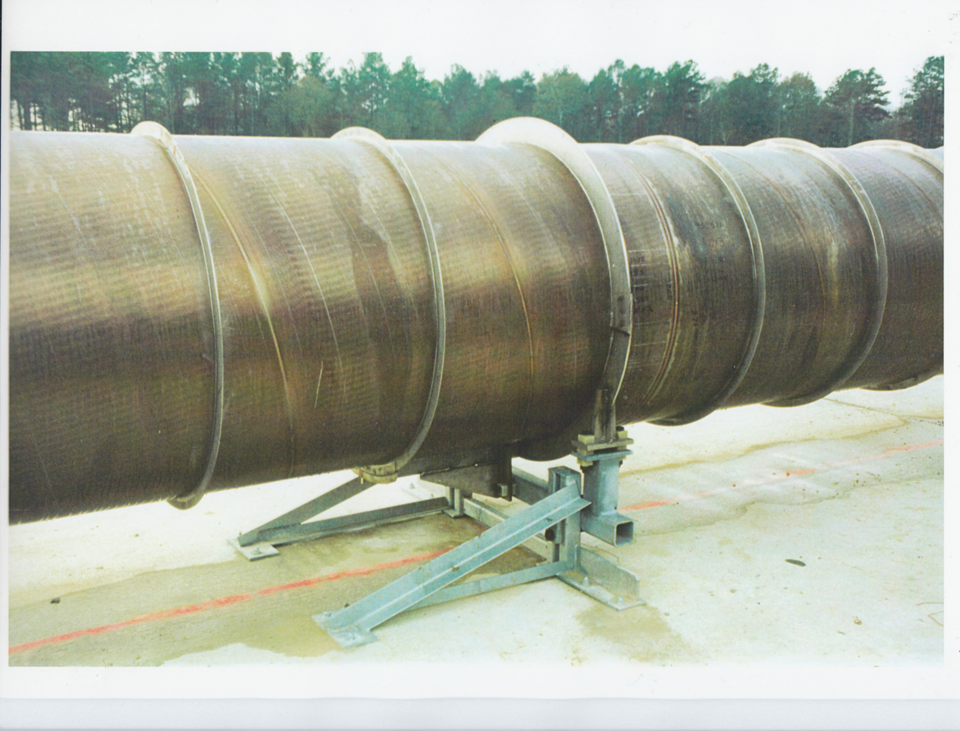
\includegraphics[width = 7 cm, height = 5 cm]{images.tex/BEAM_TUBE_SEGMENT.png}}
    \qquad
    \subfloat[]{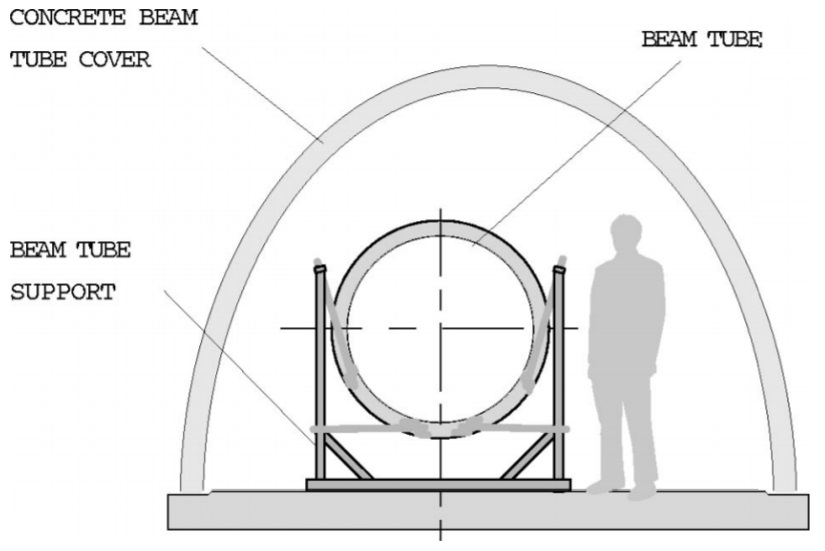
\includegraphics[width = 7 cm, height = 5 cm]{images.tex/C.S view of ligo arm.jpg}}
    \caption{(a) LIGO Beam tube. Source :- \cite{vacuum} (b) C.S view of beam tube. Source:- \cite{althouse2001precision}}
\end{figure}

\subsubsection{Laser system}

The laser used in LIGO has active material to be Nd-YAG (Neodymium - Yttrium Aluminium Garnet) and diode as the pump. Initially the laser output is $4\,W$ and wavelength of lasing light is $808\,nm$ wheich is in near infrared range. This light travels through Non-Planar Ring Oscillator (NPRO), from which a $2\,W$, $1064\,nm$ light called seed beam is generated. This is the laser which will be amplified and begins it's journey in LIGO interferometer. The seed beam is then passed through a Master-Oscillator Power Amplifier (MOPA), which consists of four thin rods of $3\,mm$ thick and $5\,cm$ long which is made similar to glass, using Nd, Y, Li and F$^{-}$. The laser power increases in each of these four rods and finally a 35W laser with the constant wavelength of 1064nm is obtained. It is now further amplified in a High-Power Oscillator (HPO) which is similar to MOPA. This results in an immensely powerful light of 200W. \cite{laser} 

\begin{figure}[h]
    \centering
    \subfloat[]{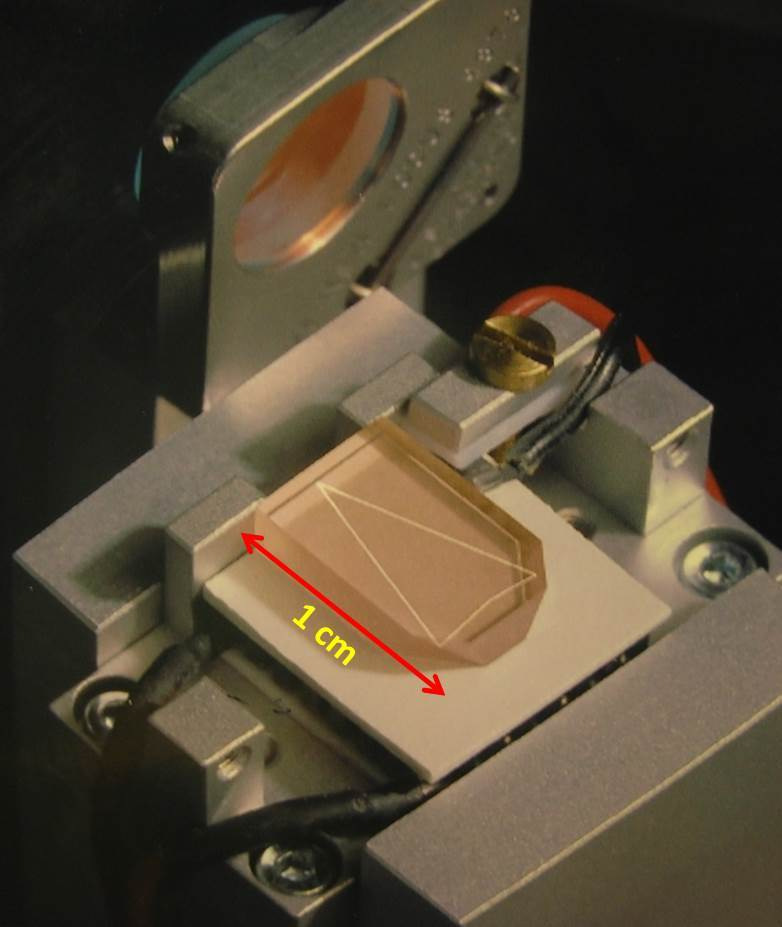
\includegraphics[width = 4.5 cm, height = 5 cm]{images.tex/NPRO.jpg}}
    \qquad
    \subfloat[]{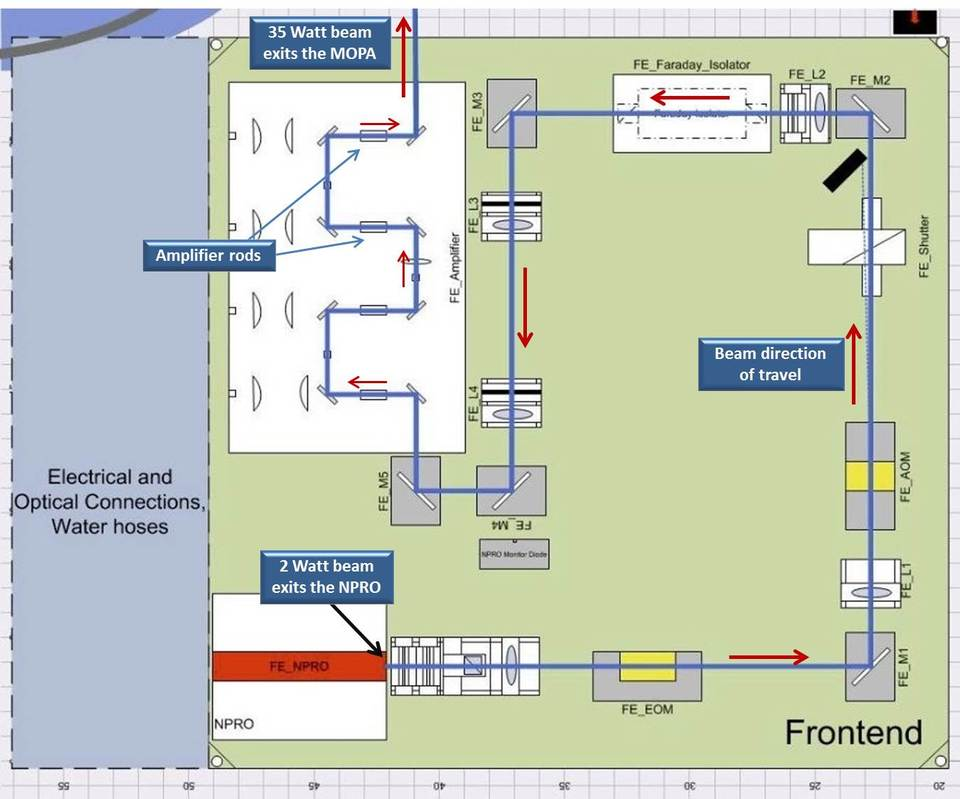
\includegraphics[width = 8.5 cm, height = 5 cm]{images.tex/Laser amplification.jpg}}
    \caption{(a) NPRO crystal. (b) schematic representation of laser amplification. \cite{laser}}
\end{figure}


\subsubsection{Beam Splitter and Mirrors}

Each arm carries two fully reflecting mirrors at its ends and a partially reflecting mirror called as Beam splitter is present at the common vertex of the arms. The space between the mirrors forms Fabry-Perot cavity. The light travels 4$km$ from one end to other, but this cavity makes the laser light to reflect approximately 300 times, so apparently the laser travels a total of $1200\,km$, this increases the laser power to $750\, kW$. The mirrors are coated extensively to nanometer smoothness (i.e the imperfections on the surface of mirror is in the order of nanometers). This is required to make the system so precise to detect even very feeble GWs. \cite{mirrors}

\begin{figure}[h]
    \centering
    \subfloat[]{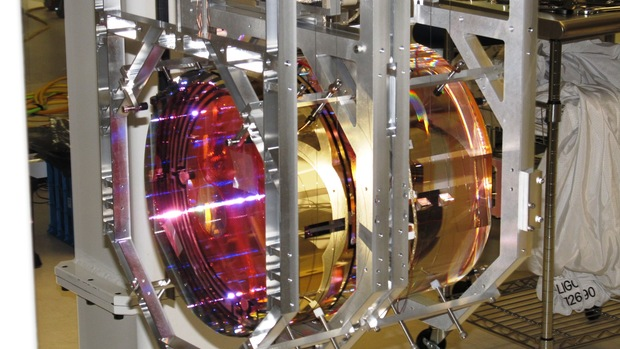
\includegraphics[width = 7 cm, height = 5 cm]{images.tex/LIGO_mirror.jpeg}}
    \qquad
    \subfloat[]{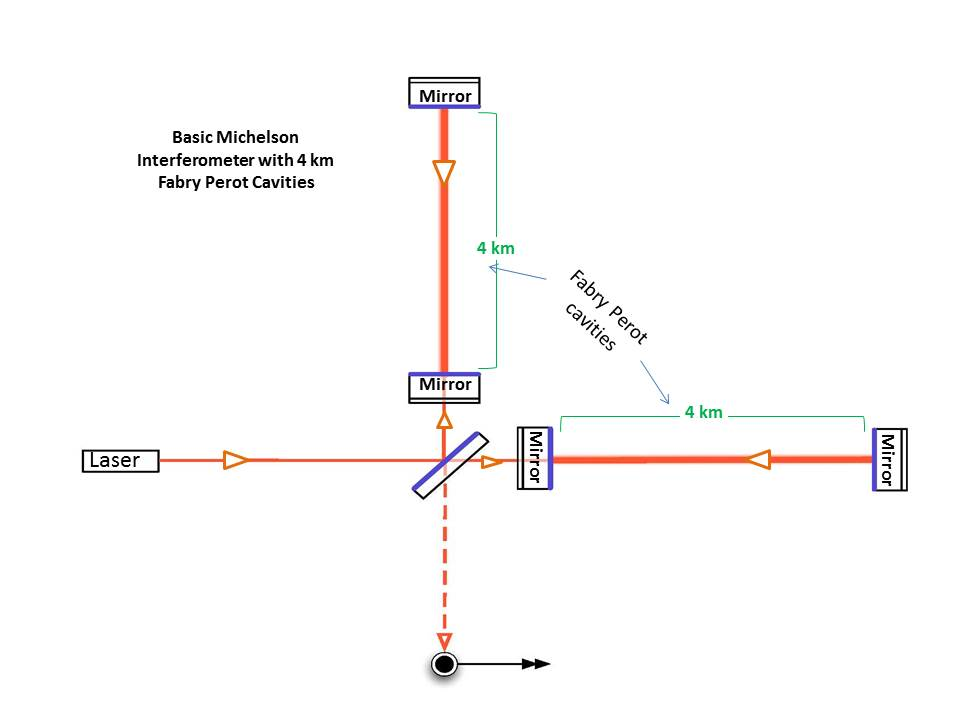
\includegraphics[width = 7 cm, height = 5.5 cm]{images.tex/Fabry Perot cavity.jpg}}
    \caption{(a) Fully reflecting mirror.\cite{mirrors} (b) Fabry-Perot cavity. \href{https://www.ligo.caltech.edu/page/ligos-ifo}{Source}}
\end{figure}


\subsubsection{Test mass and Photo-detector}

The fully reflecting mirrors are $40 \,kg$ each with thickness of $20\,cm$ and width of $34\,cm$. They act as test masses and are at 4 kilometers away from each other. This test mass is one among three other mass which are hung to a quadruple suspension system aided by silica fibers. They reduce the effect of noise vibration by 100 million times by the time it reaches the mirrors. This acts as a passive seismic isolation system. \cite{mirrors} Then finally the last component is the photo detector. Since the wavelength of operational laser is $1064\,\nm$, which lies in infrared spectrum, the photo detector should work in the infrared region. LIGO uses Broad Band Photo Detector (BBPD) which is built around a low capacitive, series resistant silicon photo-diode "FFD-100", and coupled to a $50\,\Omega$  Radio frequency amplifier called Teledyne Cougar AP389. \cite{BBPD}

\pagebreak

\subsection{Working of LIGO}

\subsubsection{Working of laser system}

To operate LIGO at its fullest potential, we need an immensely powerful laser. In order to obtain such a laser beam, it must undergo multiple stages of amplification. Initially Nd-YAG laser produces a beam in the near-infrared region of the electromagnetic spectrum at 1064 $nm$. then the beam passes through Non-Planar Ring Oscillator (NPRO), Master-Oscillator Power Amplifier (MOPA) which consists of four thin rods and finally through High-Power Oscillator (HPO). Thus a powerful laser of power $200\,W$, with wavelength $1064\,nm$ is obtained. 

\subsubsection{Working of Fabry-Perot cavity and Beam splitter}

Then the powerful collimated light beam incidents on a power recycling mirror followed by a beam splitter. The partially reflecting beam splitter splits the light into the $4\,km$ long ultra-high vacuum chambers which are present orthogonal to each other. The laser beam is spread to a diameter of 6cm when it reaches each mirror reducing the thermal effects of heating the mirror surface. The Fabry-Perot cavities make the light to reflect $\approx 300$ times which increases the laser power to $100\,kW$. Thus as the laser accumulates power gradually, after a certain value the beam splitter allows the laser beam to pass through it towards the photo-detector. The interferometer is designed such that these two coherent light beams from the perpendicular arms recombine at the beam splitter almost exactly out of phase thereby mostly cancelling the output signal when the two arms are of the same length, and the photo detector shouldn't receive any light if no disturbances are present. However, this is not the scenario if a gravitational wave passes nearby. \cite{Interferometer}

\begin{figure}[h]
    \centering
    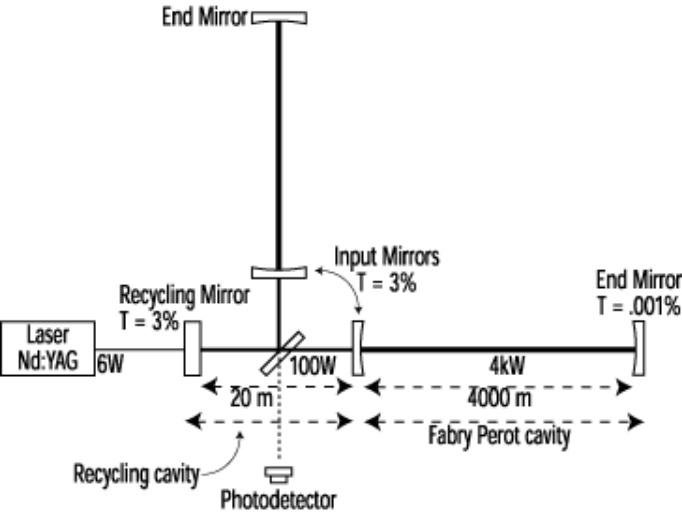
\includegraphics[scale=0.7]{images.tex/Working of Fabry-Perot cavity.jpg}
    \caption{Working of Fabry-Perot cavity. Source :- \href{https://spie.org/news/ligo-researchers-design-complex-device-to-detect-infinitesimal-changes?SSO=1}{spie.org}}
\end{figure}

\subsubsection{Working of Interferometer when gravitational wave passes}

As we saw the effect of gravitational waves, which stretch the space in one direction and compress it in the perpendicular direction. Hence, when the gravitational wave passes through the arms of LIGO, they will be subjected to compressing and stretching strain, so if the length of one arm increases, simultaneously length of other arm decreases. Even the laser light get compressed and stretched which alters the phase difference between the perpendicular light beams which causes a variation in the effective length travelled by the laser beam. Hence when the light recombine neither destructively nor constructively, where the resultant amplitude decides the intensity (I) of light that will be detected finally according to the relation

\begin{equation}
     I \propto (A_1)^2 + (A_2)^2 + 2(A_1)(A_2)\text{cos}(\Delta \phi)
\end{equation}

where $A_1$ and $A_2$ are the amplitudes of laser from LIGO's arms and $\Delta \phi$ is the phase difference between the interfering light beams. 

\begin{figure}[h]
    \centering
    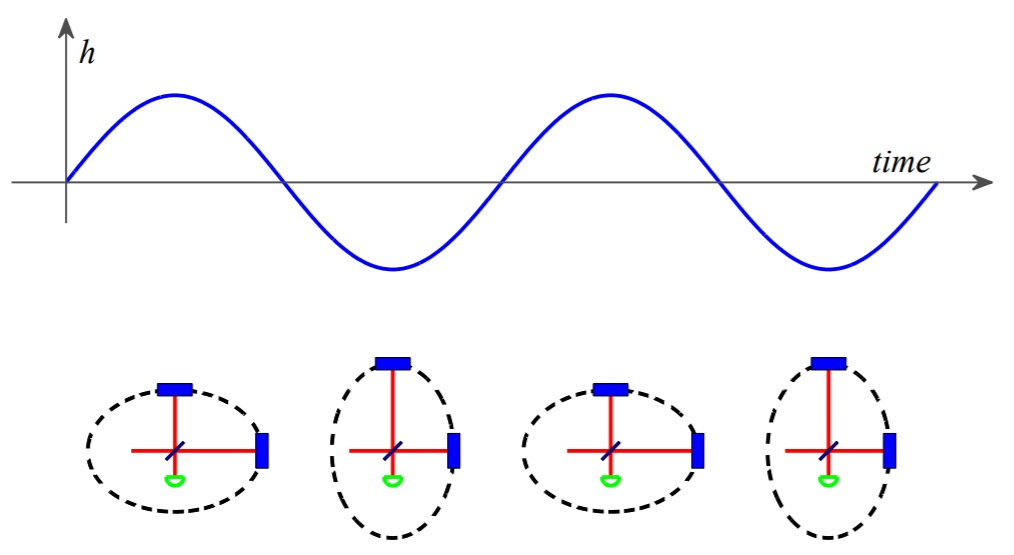
\includegraphics[scale =0.6]{images.tex/GW effect on LIGO arm.jpg}
    \caption{Gravitational wave effect on LIGO arms. Source :- \href{https://www.semanticscholar.org/paper/Broadband-Measurement-and-Reduction-of-Quantum-in-Cripe/ffe14b1a34d504599fa81c817bbb9aef5385c06c}{Semanticscholar.org} \cite{Cripe2020BroadbandMA}}
\end{figure}

So if there is no disturbance, then the arms will be intact, thus the light interfere destructively and the intensity of light detected by the photo detector will be zero, thus no signal is recorded. But if gravitational wave passes, due to change in length of LIGO arms, a phase difference will be created such that the light will interfere partially, thus the intensity of light will fluctuate. The frequency of fluctuation of intensity will be a function of time which will be calculated by the photo detector and that can be converted to the strain caused on the arms which in turn will be a function of frequency. This will be calculated by the computers which is generally shown as the wave form of the detected gravitational wave. 

\begin{figure}[h]
    \centering
    \subfloat[]{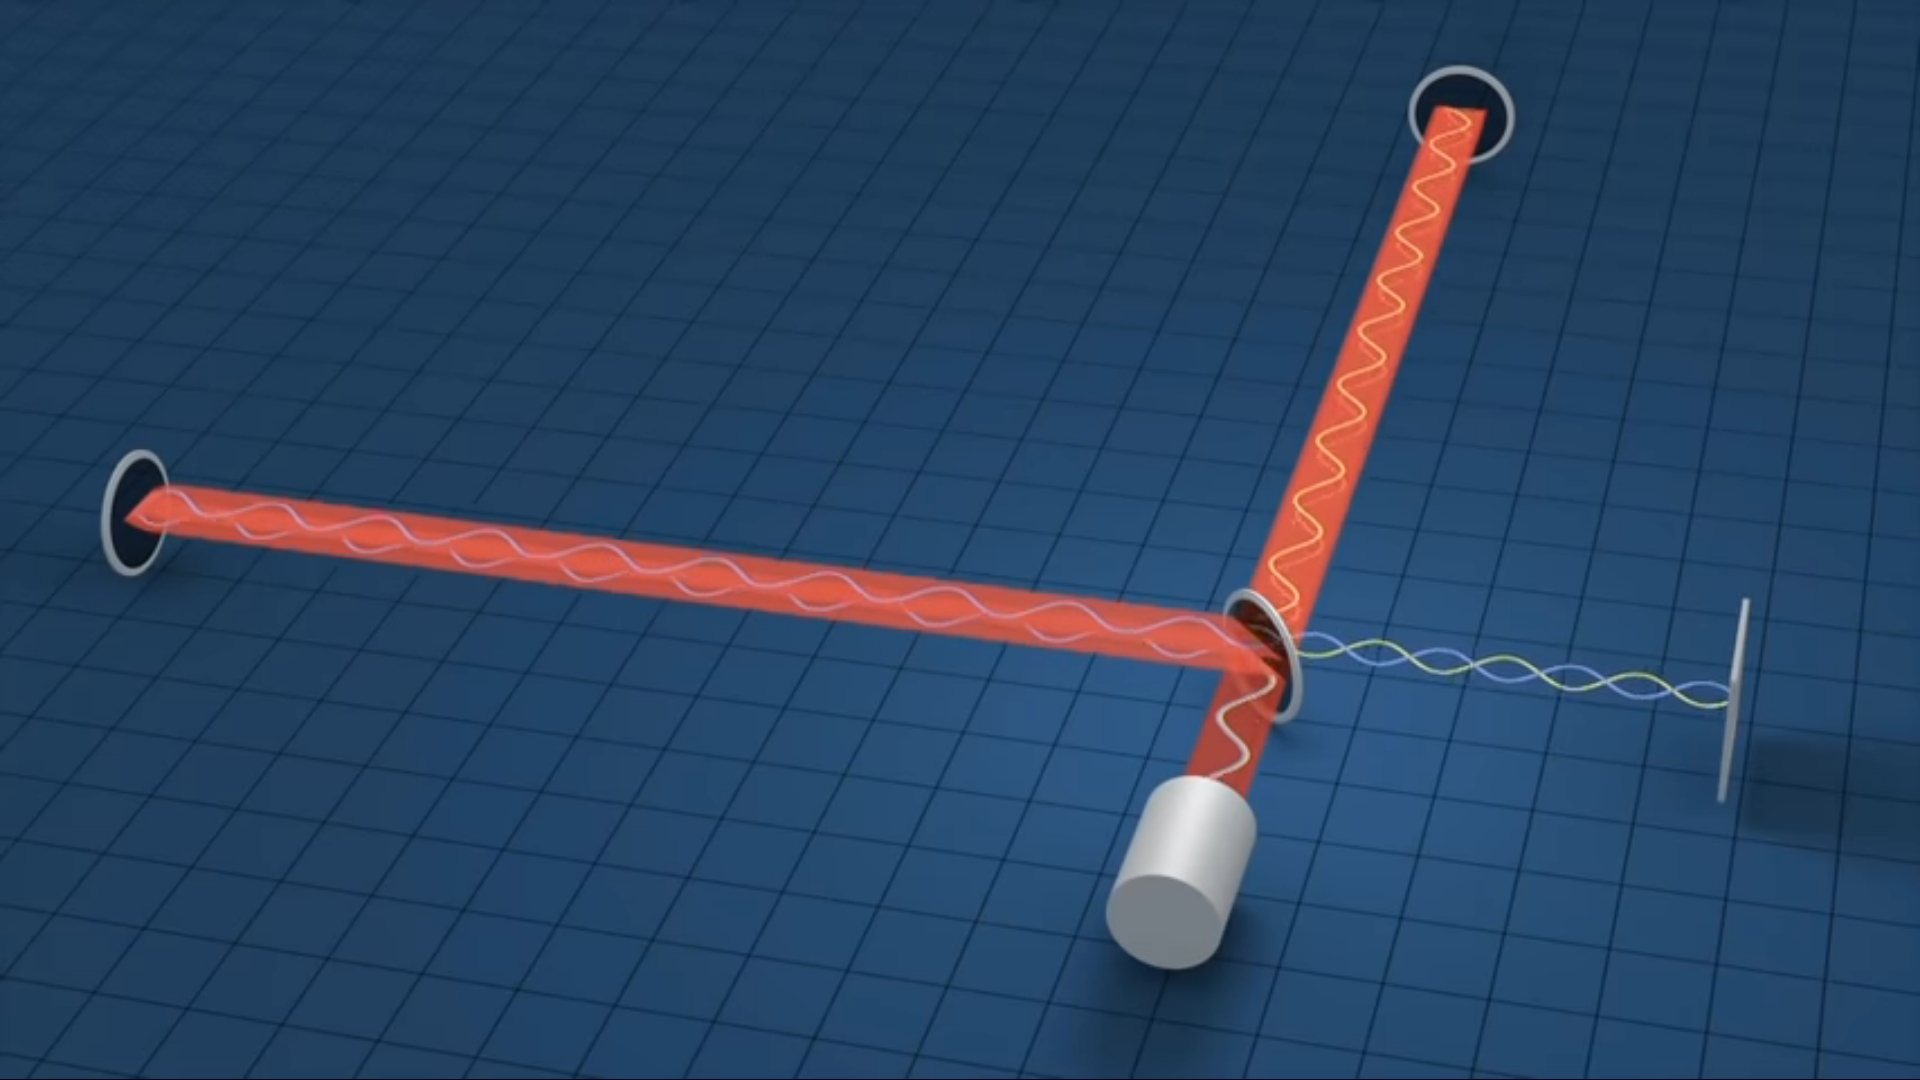
\includegraphics[width = 5.5 cm, height = 4 cm]{images.tex/Initial condition.png}}
    \qquad
    \subfloat[]{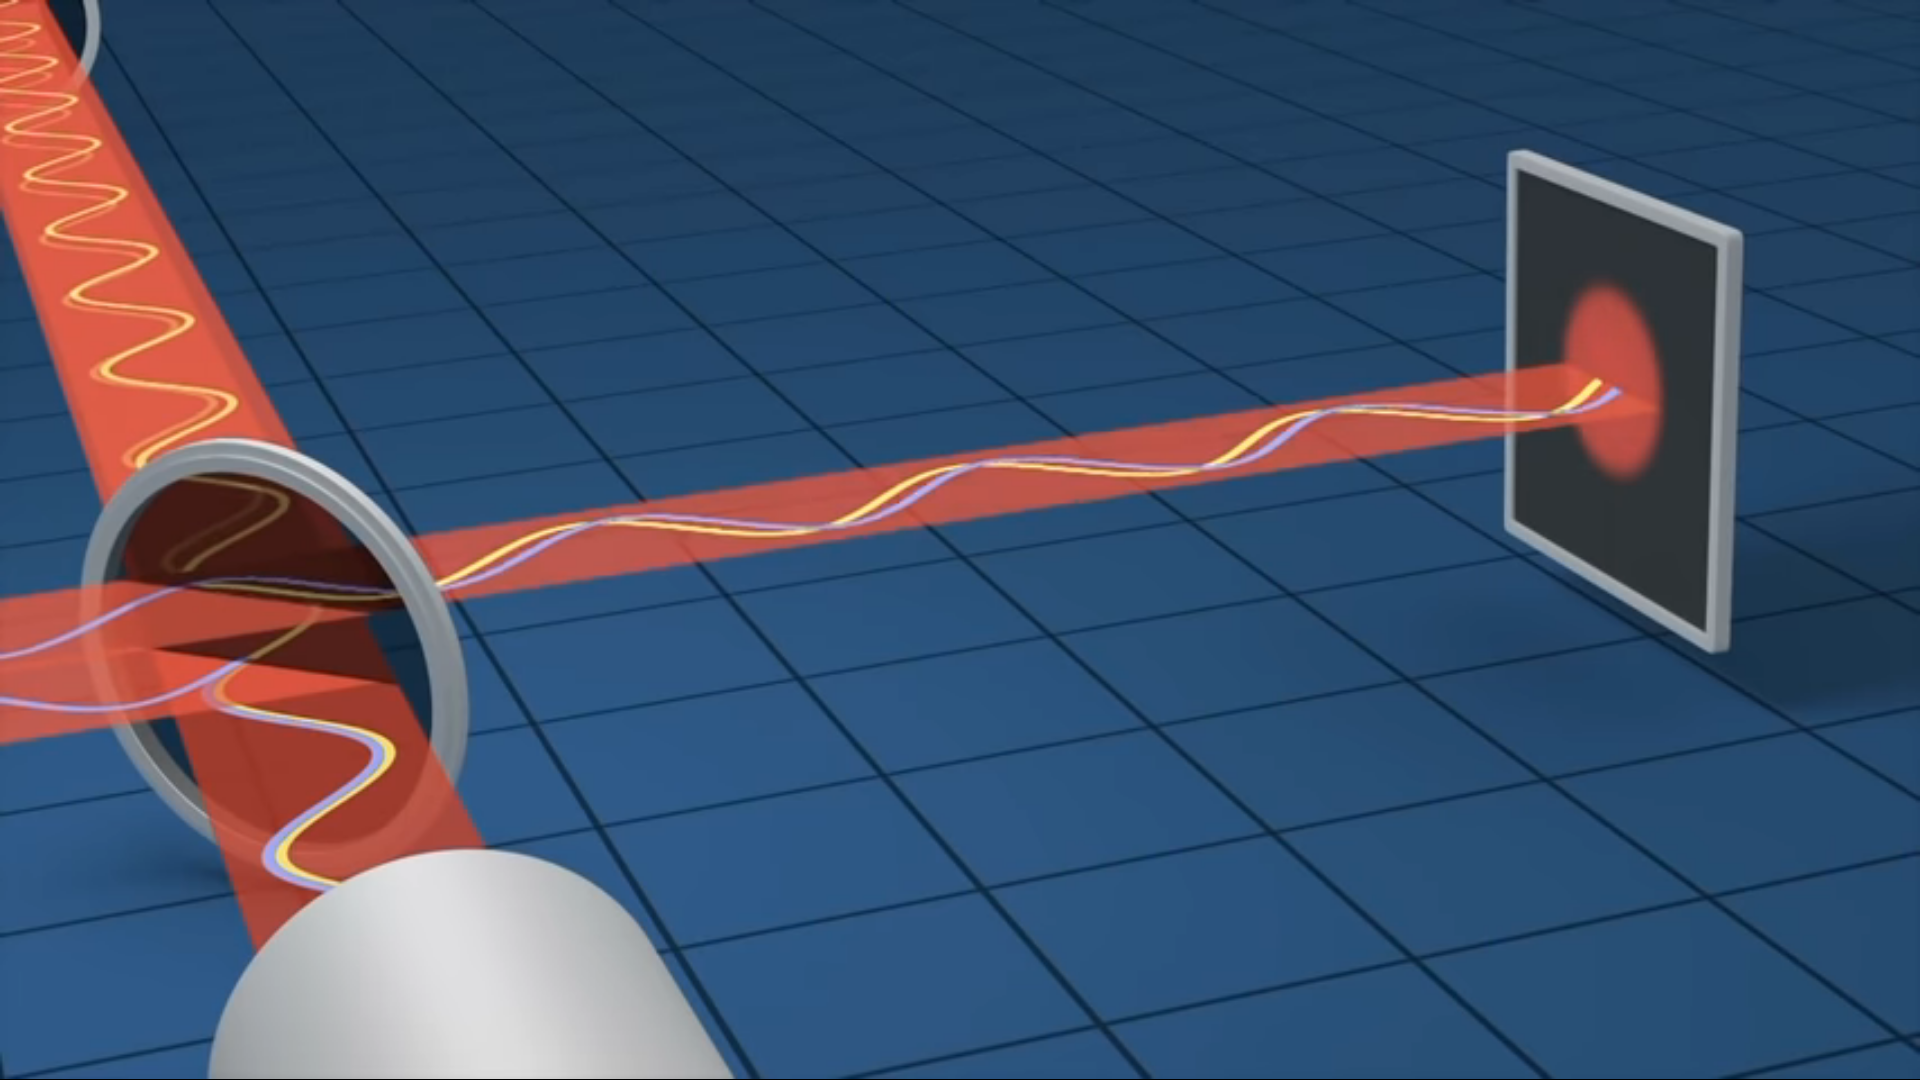
\includegraphics[width = 5.5 cm, height = 4 cm]{images.tex/Constructive.png}}
    \qquad
    \subfloat[]{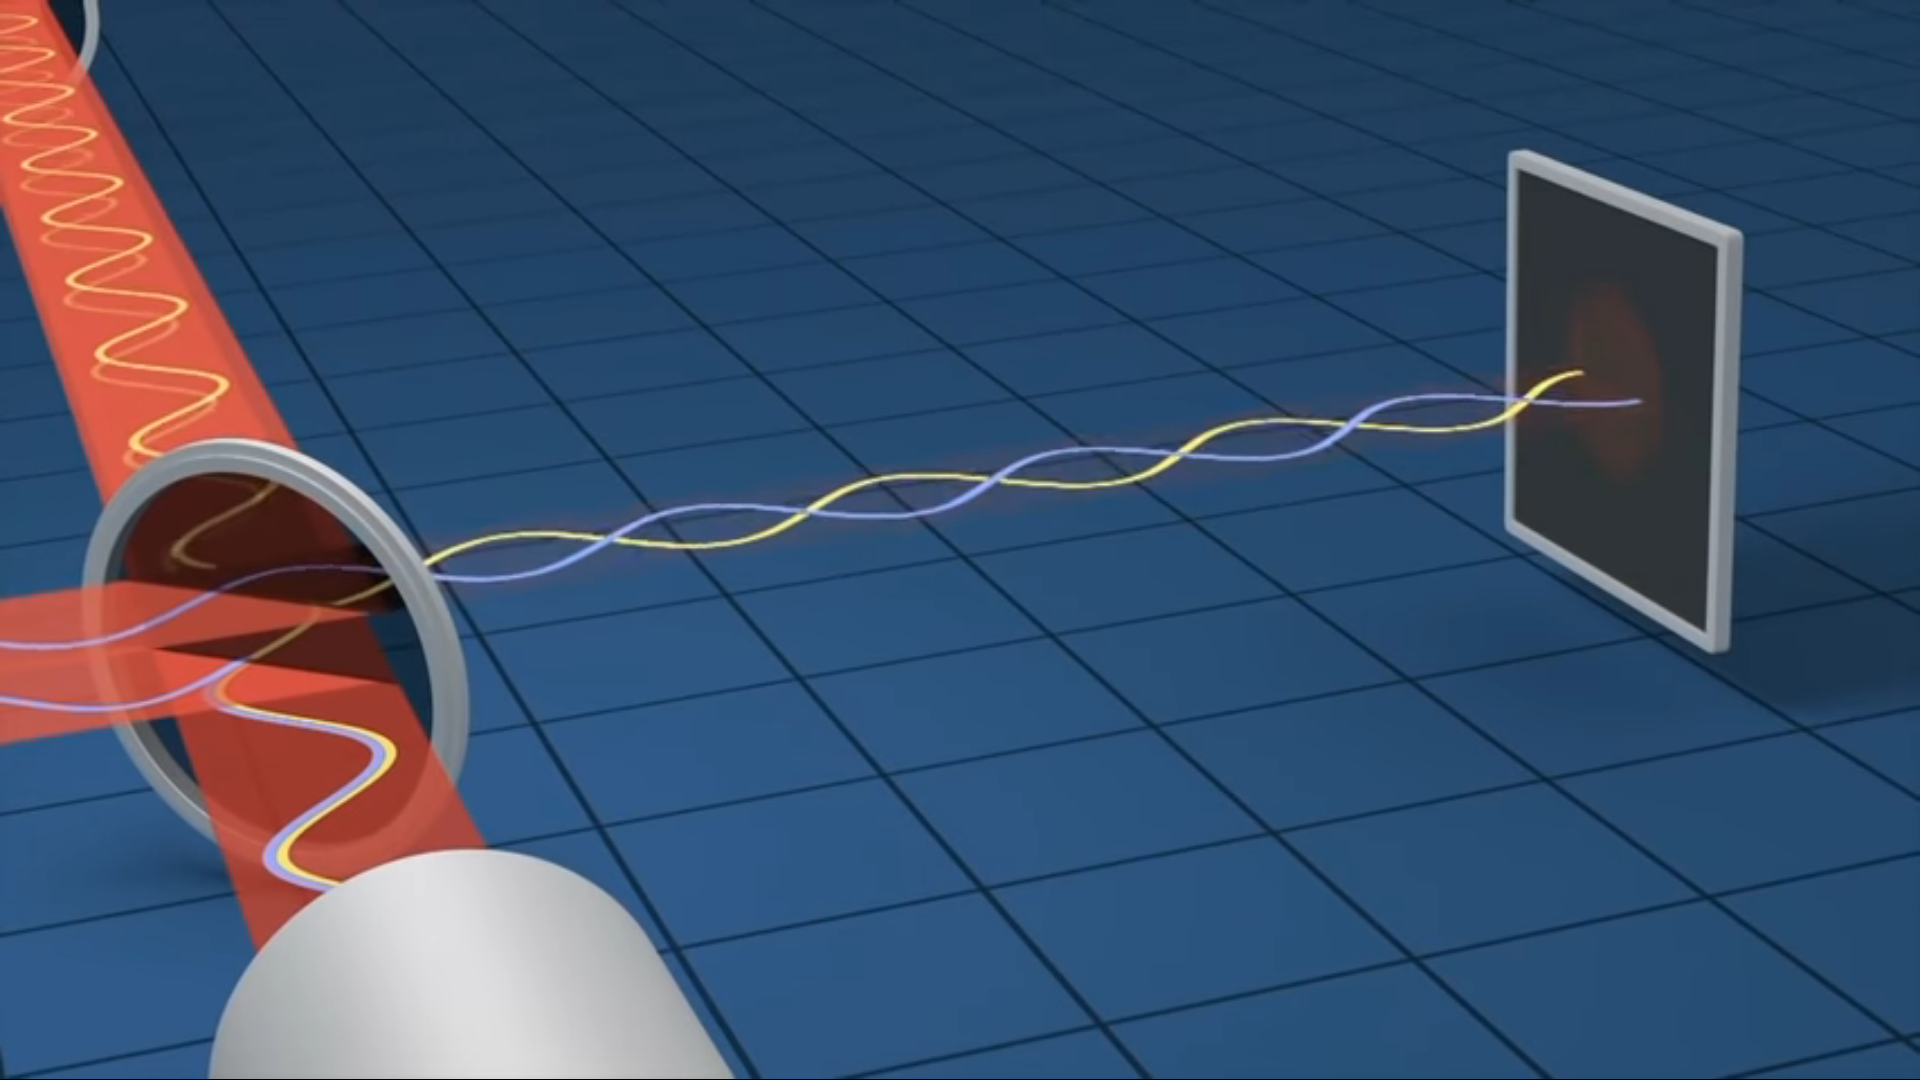
\includegraphics[width = 5.5 cm, height = 4 cm]{images.tex/Destructive.png}}
    \qquad
    \subfloat[]{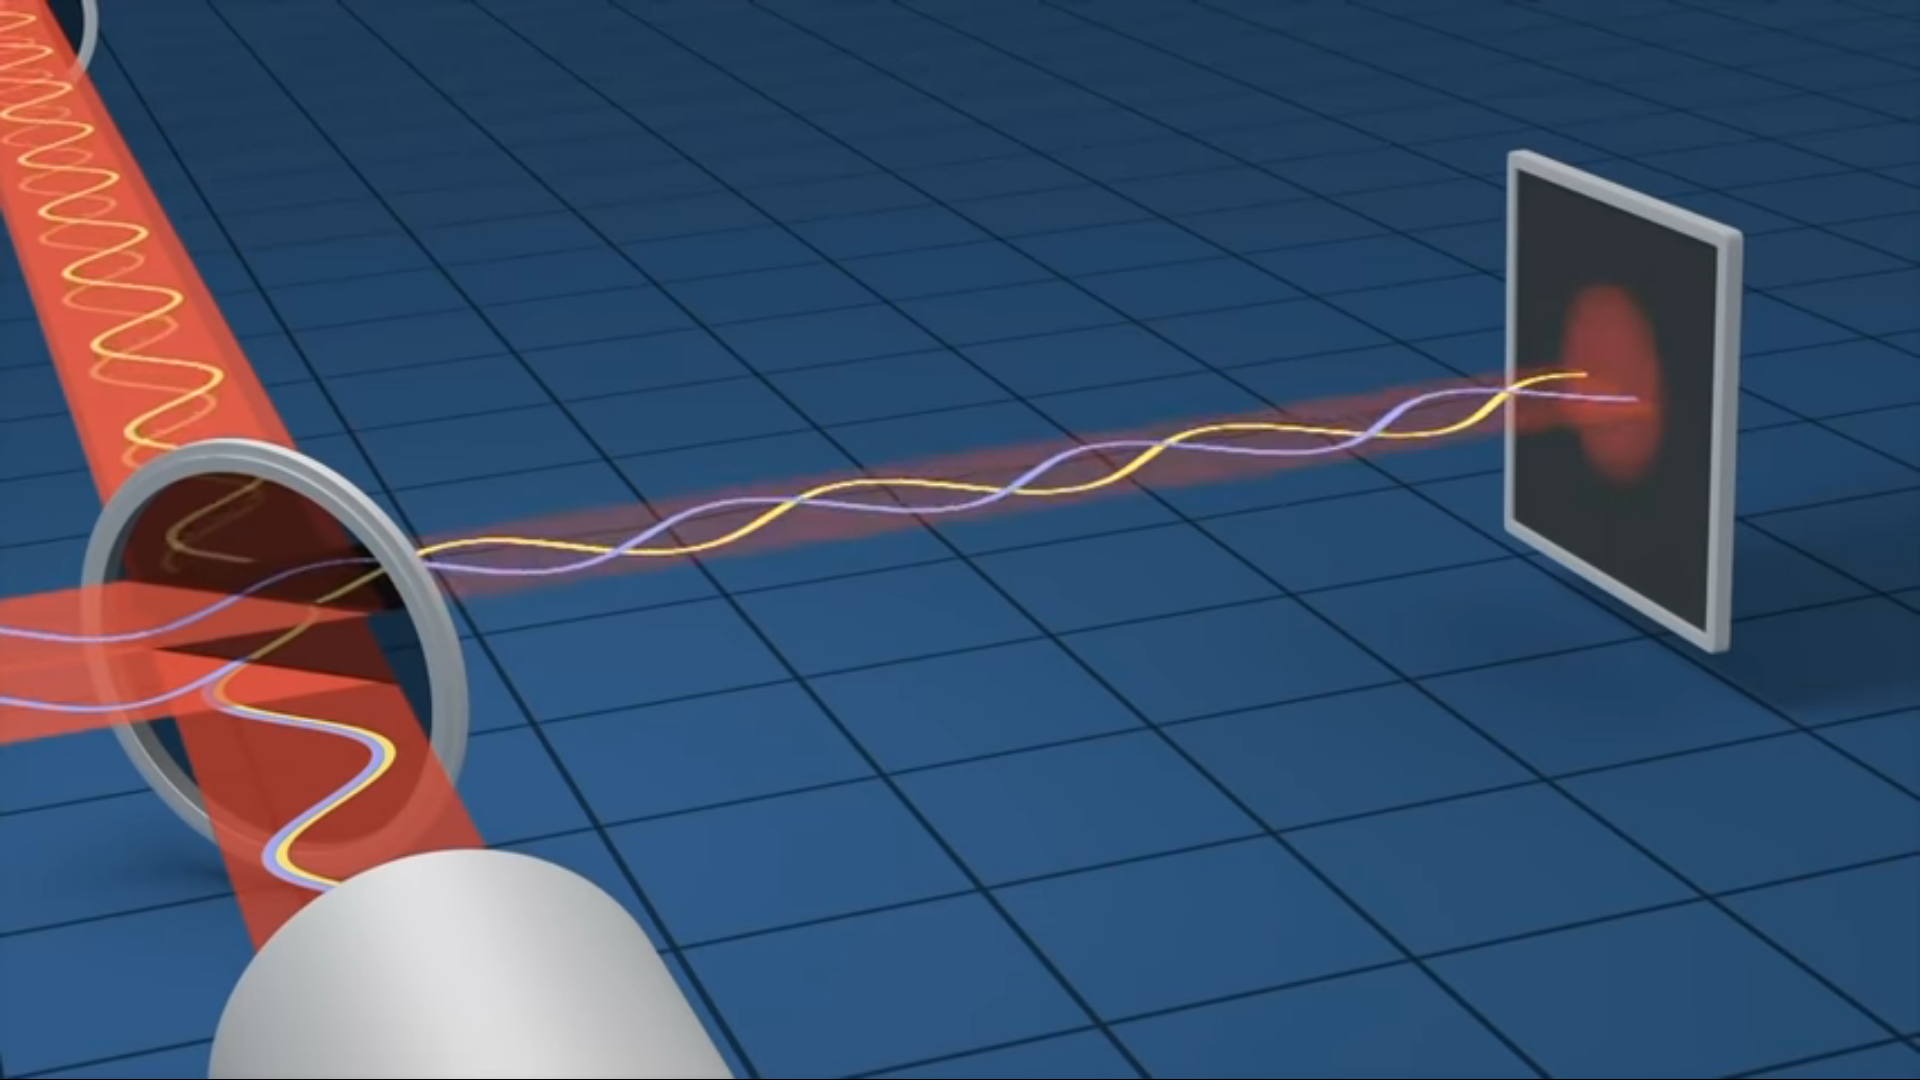
\includegraphics[width = 5.5 cm, height = 4 cm]{images.tex/Intermediate.png}}
    \caption{(a) Initial Condition (b) Constructive interference.\\
    (c) Destructive interference (d) Partial interference}
\end{figure}

But apart from gravitational waves, there are other disturbances also. Like earthquakes which can also influence the interference pattern. To avoid this as much, the whole system is evacuated. Other measures are also taken to dampen these vibrations which are described in noise cancellation.

\pagebreak

\input{8 LIGO.tex/8.4 Noise_cancellation}
\input{8 LIGO.tex/8.5 Signal_extraction_conversion}

\section{Detection of Gravitational waves using LIGO }
\input{9 Detection_by_ligo.tex/9.1 First Observation}
\subsection{Some Detections of LIGO}

\subsubsection{GW190814}

Two advanced-LIGO detectors (Hanford, Washington and Livingston, Louisiana, USA) and the advanced-Virgo detector (Cascina, Italy), have detected gravitational waves from the inspiral and merger of a stellar-mass black hole and another compact object on 14th August, 2019 at 21:10:39 UTC. It has been named as GW190814 as the date suggests.

\begin{figure}[h]
    \centering
    \includegraphics[scale = 0.91]{images.tex/GW190814.jpg}
    \caption{Frequency Vs Time data of GW190814 in three observatories. Source:- \href{https://en.wikipedia.org/wiki/GW190814}{Wikipedia}}
\end{figure}

While the mass of one component of this binary could range from 22.2 to 24.3 $M_\odot$ black hole, the other component which was of 2.6 solar mass could be either a low-mass black hole or a heavy neutron star. The masses of the objects before merging differed by a factor of 9. This makes it the most extreme mass ratio known for some GW event. The source of this GW was in a small patch of sky of around 20 square degrees. Even after doing so much research, the counterpart of the black hole which was in the inspiral mechanism wasn’t observed. It can be that, either black hole consumed the neutron star completely or both were black holes. Had we observe an electromagnetic counterpart, which may not have happened due to a number of reasons, we could say the smaller object is mostly neutron star. 

\pagebreak

\subsubsection{GW170817}

On 17th August, 2017, LIGO and Virgo detectors observed a gravitational wave named as GW170817. It is known to be produced by two neutron stars merging into each other while spiralling closer and closer. The aftermath of this GW was observed by around 70 observatories on 7 continents as well as through space, across the electromagnetic spectrum, marking a significant breakthrough for multi-messenger astronomy. The discovery and subsequent observations of GW170817 got Breakthrough of the Year award for 2017 by the journal Science.

\begin{figure}[h]
    \centering
    \includegraphics[scale=0.78]{images.tex/GW170817_observatories.png}
    \caption{Frequency Vs Time data of GW170817 in three observatories. Source:- \href{https://en.wikipedia.org/wiki/GW170817}{Wikipedia}}
\end{figure}

The component masses of the binary are inferred to be between 1.17 and 1.60 $M_\odot$. After merging it makes the mass of about 2.74 $M_\odot$. The gravitational wave signal lasted for about 100 seconds. It started with a frequency of 24 $Hz$. It  inspiralled for around 3,000 cycles. The amplitude and frequency increased to a few hundred hertz as both the objects came nearer in the typical inspiral chirp pattern. Lastly, it ended with the collision at 12:41:04.4 UTC which was received as a signal in the interferometer. At first, it arrived at the Virgo detector in Italy. After 22 milliseconds, detectors at the LIGO-Livingston detector in Louisiana, United States got the signals. After another 3 milliseconds, the waves reached at the LIGO-Hanford detector in the state of Washington, United States. It was then compared with a prediction from the general theory of relativity given by Einstein to analyse it further. The source was localised within a sky region of 28\degree square which has a probability of 90\%.

A gamma-ray burst, GRB 170817A was detected. It lasted for $\approx$ 2 seconds. It was detected by Fermi and INTEGRAL spacecrafts. This bursts began at 1.7 seconds after the signal received denoting the merge of the objects. It's a hypothesis that neutron star mergers cause gamma-ray bursts which gets confirmed with this merger.

\pagebreak

\subsubsection{GW190521}

LIGO-VIRGO detectors detected a short signal from a binary black hole merger
on May 21,2019 at 03:02:29 UTC. The event occurred at a luminosity distance $5.3_{-2.6}^{+2.4}\,Gpc$ with a red shift of $0.82_{-0.34}^{+0.28}$. The signal lasted for about 0.1 seconds long and had a peak frequency of about $60\,Hz$. Since the time period and frequency is inversely proportional to the binary’s total mass, and since the signal was so short, this could imply that in this event the most massive black holes could have collided when compared to the collisions detected so far with a total mass of $150_{-17}^{+29}\,M_\odot$. The two black holes weighed upto $85_{-14}^{+21}\, M_\odot$ and $66_{-18}^{+17} \,M_\odot$ giving rise to a $142_{-16}^{+28}\, M_\odot$ remnant black hole. \cite{GW190521_1}

\begin{figure}[h]
    \centering
    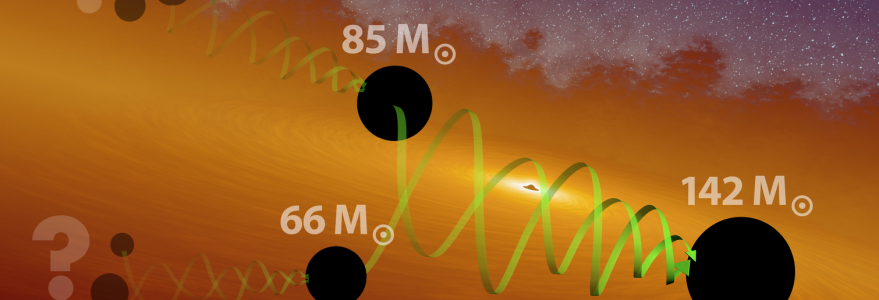
\includegraphics[scale = 0.5]{images.tex/GW190521 representation.jpg}
    \caption{Pictorial representation of GW190521 merger. Source :- \href{https://en.uw.edu.pl/virgo-and-ligo-unveil-new-and-unexpected-black-hole-populations/}{en.uw.edu.pl}}
\end{figure}

The mass of the remnant black hole is between 100 and 1000 $M_\odot$, making it the first intermediate mass black hole to be detected. Not only is the remnant black hole bizarre, but the two mergers had masses which are impossible to be directly formed by collapsing stars. This led to the theory that these kinds of black holes may be formed by merging of smaller black holes or stars can form black holes with higher masses. Regions like the galactic centre or star clusters might favour the existence of such black holes \cite{GW190521_2}. An electromagnetic counterpart was also detected but its association with the event GW190521 is uncertain. This is the first time an electromagnetic counterpart has ever been detected from the merging of black holes. The one unsolved problem here is why an electromagnetic counterpart observed as the black hole mergers do not emit light. It is approximated that the two black holes orbited a super massive black hole. After the formation of the intermediate mass black hole, it must have crossed the gaseous disk, that caused it to light up. The first largest merger and the unexplained electromagnetic counterpart are some of the most notable features.


\begin{figure}[h]
    \centering
    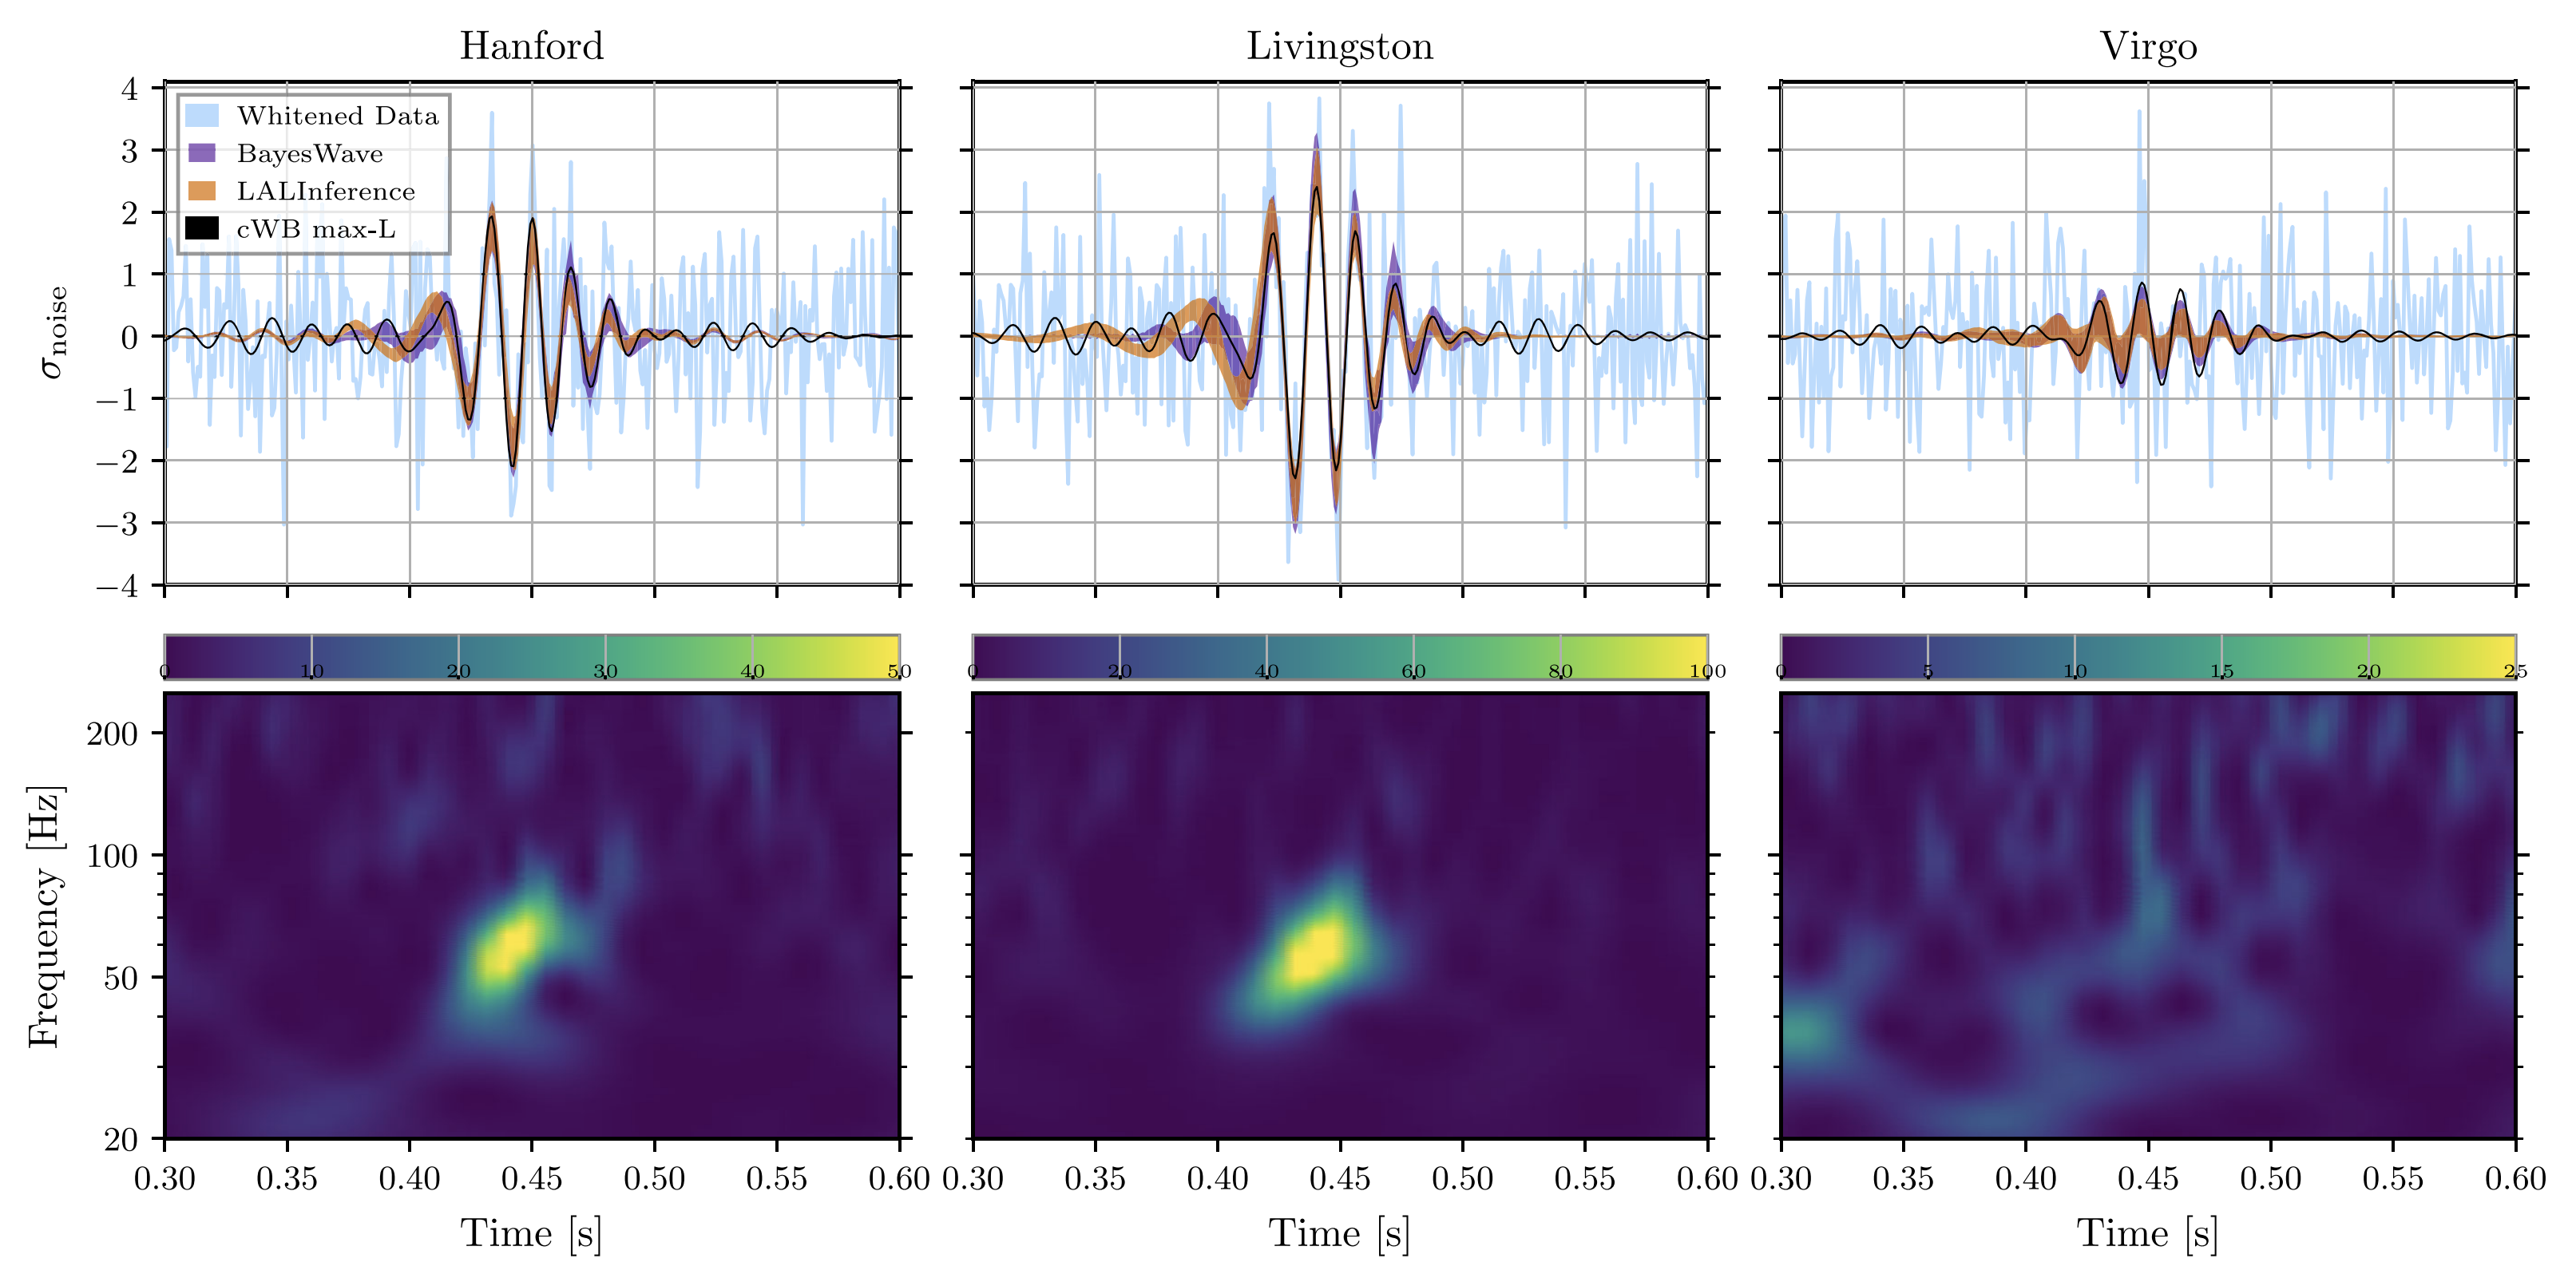
\includegraphics[width=15cm, height = 8cm]{images.tex/GW190521.png}
    \caption{Wave form of GW190521 signal. \\ Source :- \href{https://journals.aps.org/prl/abstract/10.1103/PhysRevLett.125.101102}{GW190521:A Binary Black Hole Merger with a Total Mass of 150$M_\odot$}}
\end{figure}

\pagebreak

\subsubsection{GW190425}
The signal was detected by LIGO-Livingston and VIRGO detector during the third observational run O3 on 25 April,2019 at 08:18:05 UTC whereas LIGO-Hanford was temporarily offline.The signal originated from a region of the sky which was not in plain sight for VIRGO and it lied just above the detection threshold for LIGO-Livingston. Luminosity distance of the event was 159$_{-71}^{+69}$ Mpc. \cite{GW190425_1}

\begin{figure}[htpb]
    \centering
    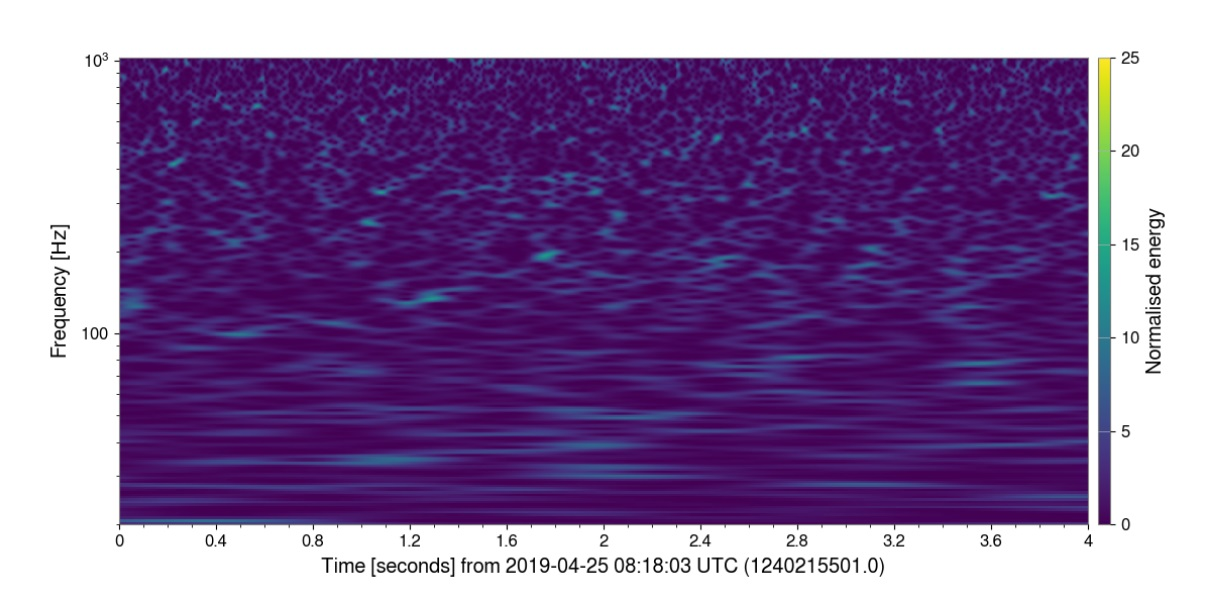
\includegraphics[scale=0.75]{images.tex/GW190425 L1.jpg}
    \caption{Signal detected by L1. Source :- \href{https://www.gw-openscience.org/eventapi/html/O3_Discovery_Papers/GW190425/v1/}{gw-openscience.org}}
    \end{figure}
    
\begin{figure}[htpb]
    \centering
    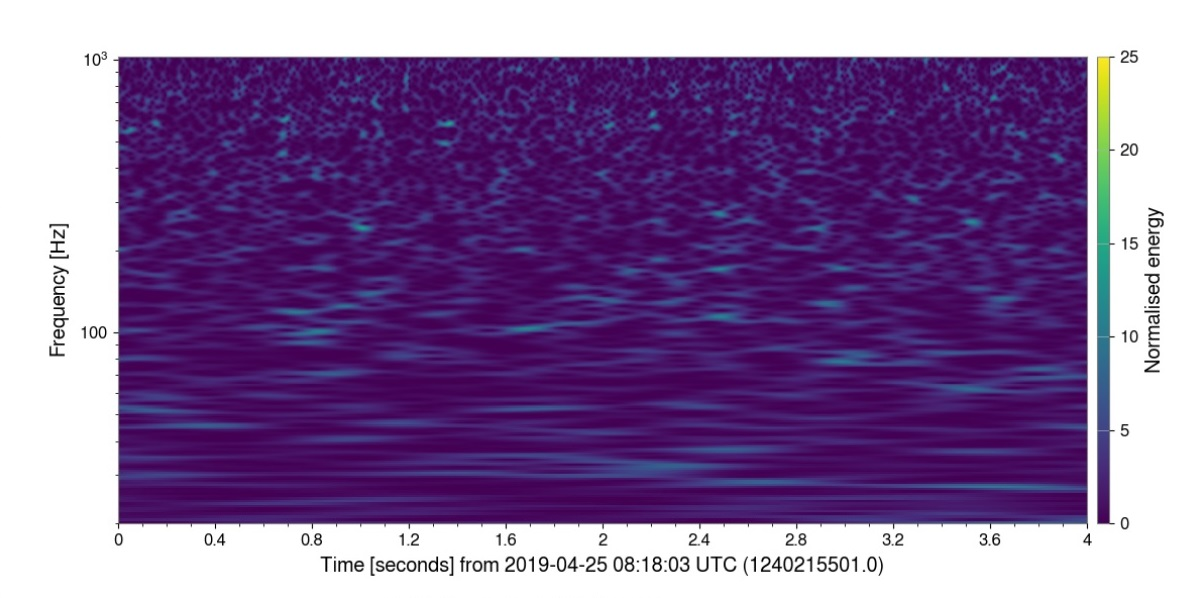
\includegraphics[scale=0.75]{images.tex/GW190425 V1.jpg}
    \caption{Signal detected by V1. Source :- \href{https://www.gw-openscience.org/eventapi/html/O3_Discovery_Papers/GW190425/v1/}{gw-openscience.org}}
\end{figure}

The mass of the mergers was estimated to be $1.61-2.52\,M_\odot$ and $1.12 - 1.68\,M_\odot$.The total mass of the compact binary was $3.4_{-0.1}^{+0.3}\, M_\odot$, greater than any known binary neutron stars. This suggests that the formation of GW190425 was different than the known binary neutron stars. One possible explanation for this is that the source consisted of a neutron star and a $4.5\,M_\odot$ helium star which evolved to form an eccentric double neutron star \cite{Romero_Shaw_2020}. Unlike the other neutron star mergers that produced electromagnetic counterparts, no such counterparts were observed for GW190425 \cite{GW190425_1}.

\pagebreak

\subsubsection{GW190412}

On 12th April, 2019 05∶30∶44 UTC, the Advanced Virgo detector and both of the Advanced LIGO detectors, detected a gravitational wave which was named GW190412. The signal was recorded with a network signal-to-noise (SNR) ratio of 19. In this event, a $30\, M_\odot$ black hole coalesced with a $8\,M_\odot$ black hole. This merger was significant because a combined Signal to Noise ratio (SNR) of 19 was found in across all three GW detectors, in addition to the BBH system being the first to be observed with an asymmetric component mass ratio.\\

While the inferred individual masses of the coalescing black holes (BHs) are each within the range of masses that have been observed before, previously detected binaries all had mass ratios $ q = \frac{m_2}{m_1}$ (with $m_1 \geq m_2$) that were according to unity. GW190412, is the first observation of Gravitational waves by LIGO from a coalescing binary with indubitably unequal masses. GWs from this event carry faint but clearly measurable evidence of radiation that oscillates at frequencies with subdominant contributions for the first time as a result of the mass asymmetry of the BBH system.

\begin{figure}[h]
    \centering
    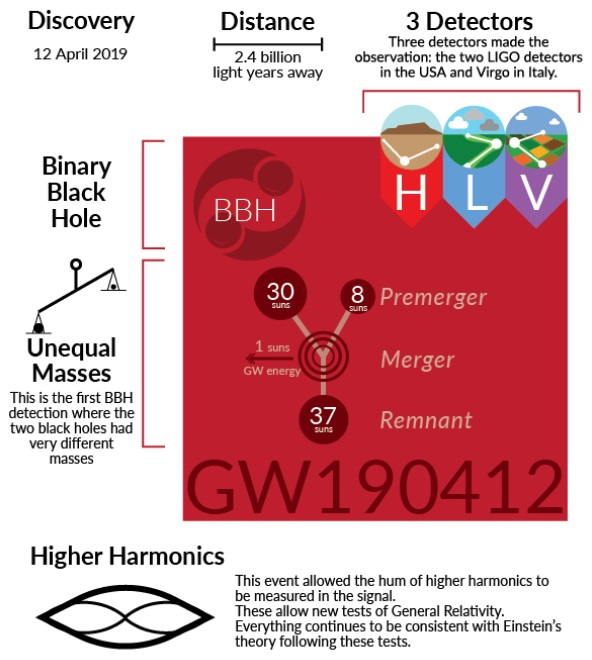
\includegraphics[scale=1.15]{images.tex/GW190412.jpg}
    \caption{Characteristics of GW190412. Source :- \href{https://www.ligo-india.in/outreach/detections/gw190412/}{LIGO-India.in}}
\end{figure}

Einstein’s Theory of General Relativity predicts that although gravitational radiation from compact binaries is dominated by a quadrupolar structure, it also contains weaker contributions from subdominant multi poles. In particular, gravitational radiation from systems with significantly asymmetric component masses consist of stronger contributions from higher multi poles. GW190412 presents strong evidence for contribution to gravitational radiation beyond the leading quadrupolar order in asymmetric systems.

\pagebreak

\subsubsection{GW170104}

GW170104, a gravitational-wave signal produced by the coalescence of a pair of stellar-mass black holes, was measured on 4th of January 2017 at 10:11:58.6 UTC by the Hanford and Livingston advanced detectors of the Laser Interferometer Gravitational-Wave Observatory with a network signal-to-noise ratio of 13 and a false alarm rate less than 1 in 70 000 years. The inferred component black hole masses are $31.2^{+8.4}_{-6.0}\,M\odot$  and $19.4^{+5.3}_{-5.9}\,M\odot$ (with 90\% credibility). The gravitational wave frequency at peak GW strain was $160$ to $199\, Hz$. \cite{PhysRevLett.118.221101}

\begin{figure}[h]
    \centering
    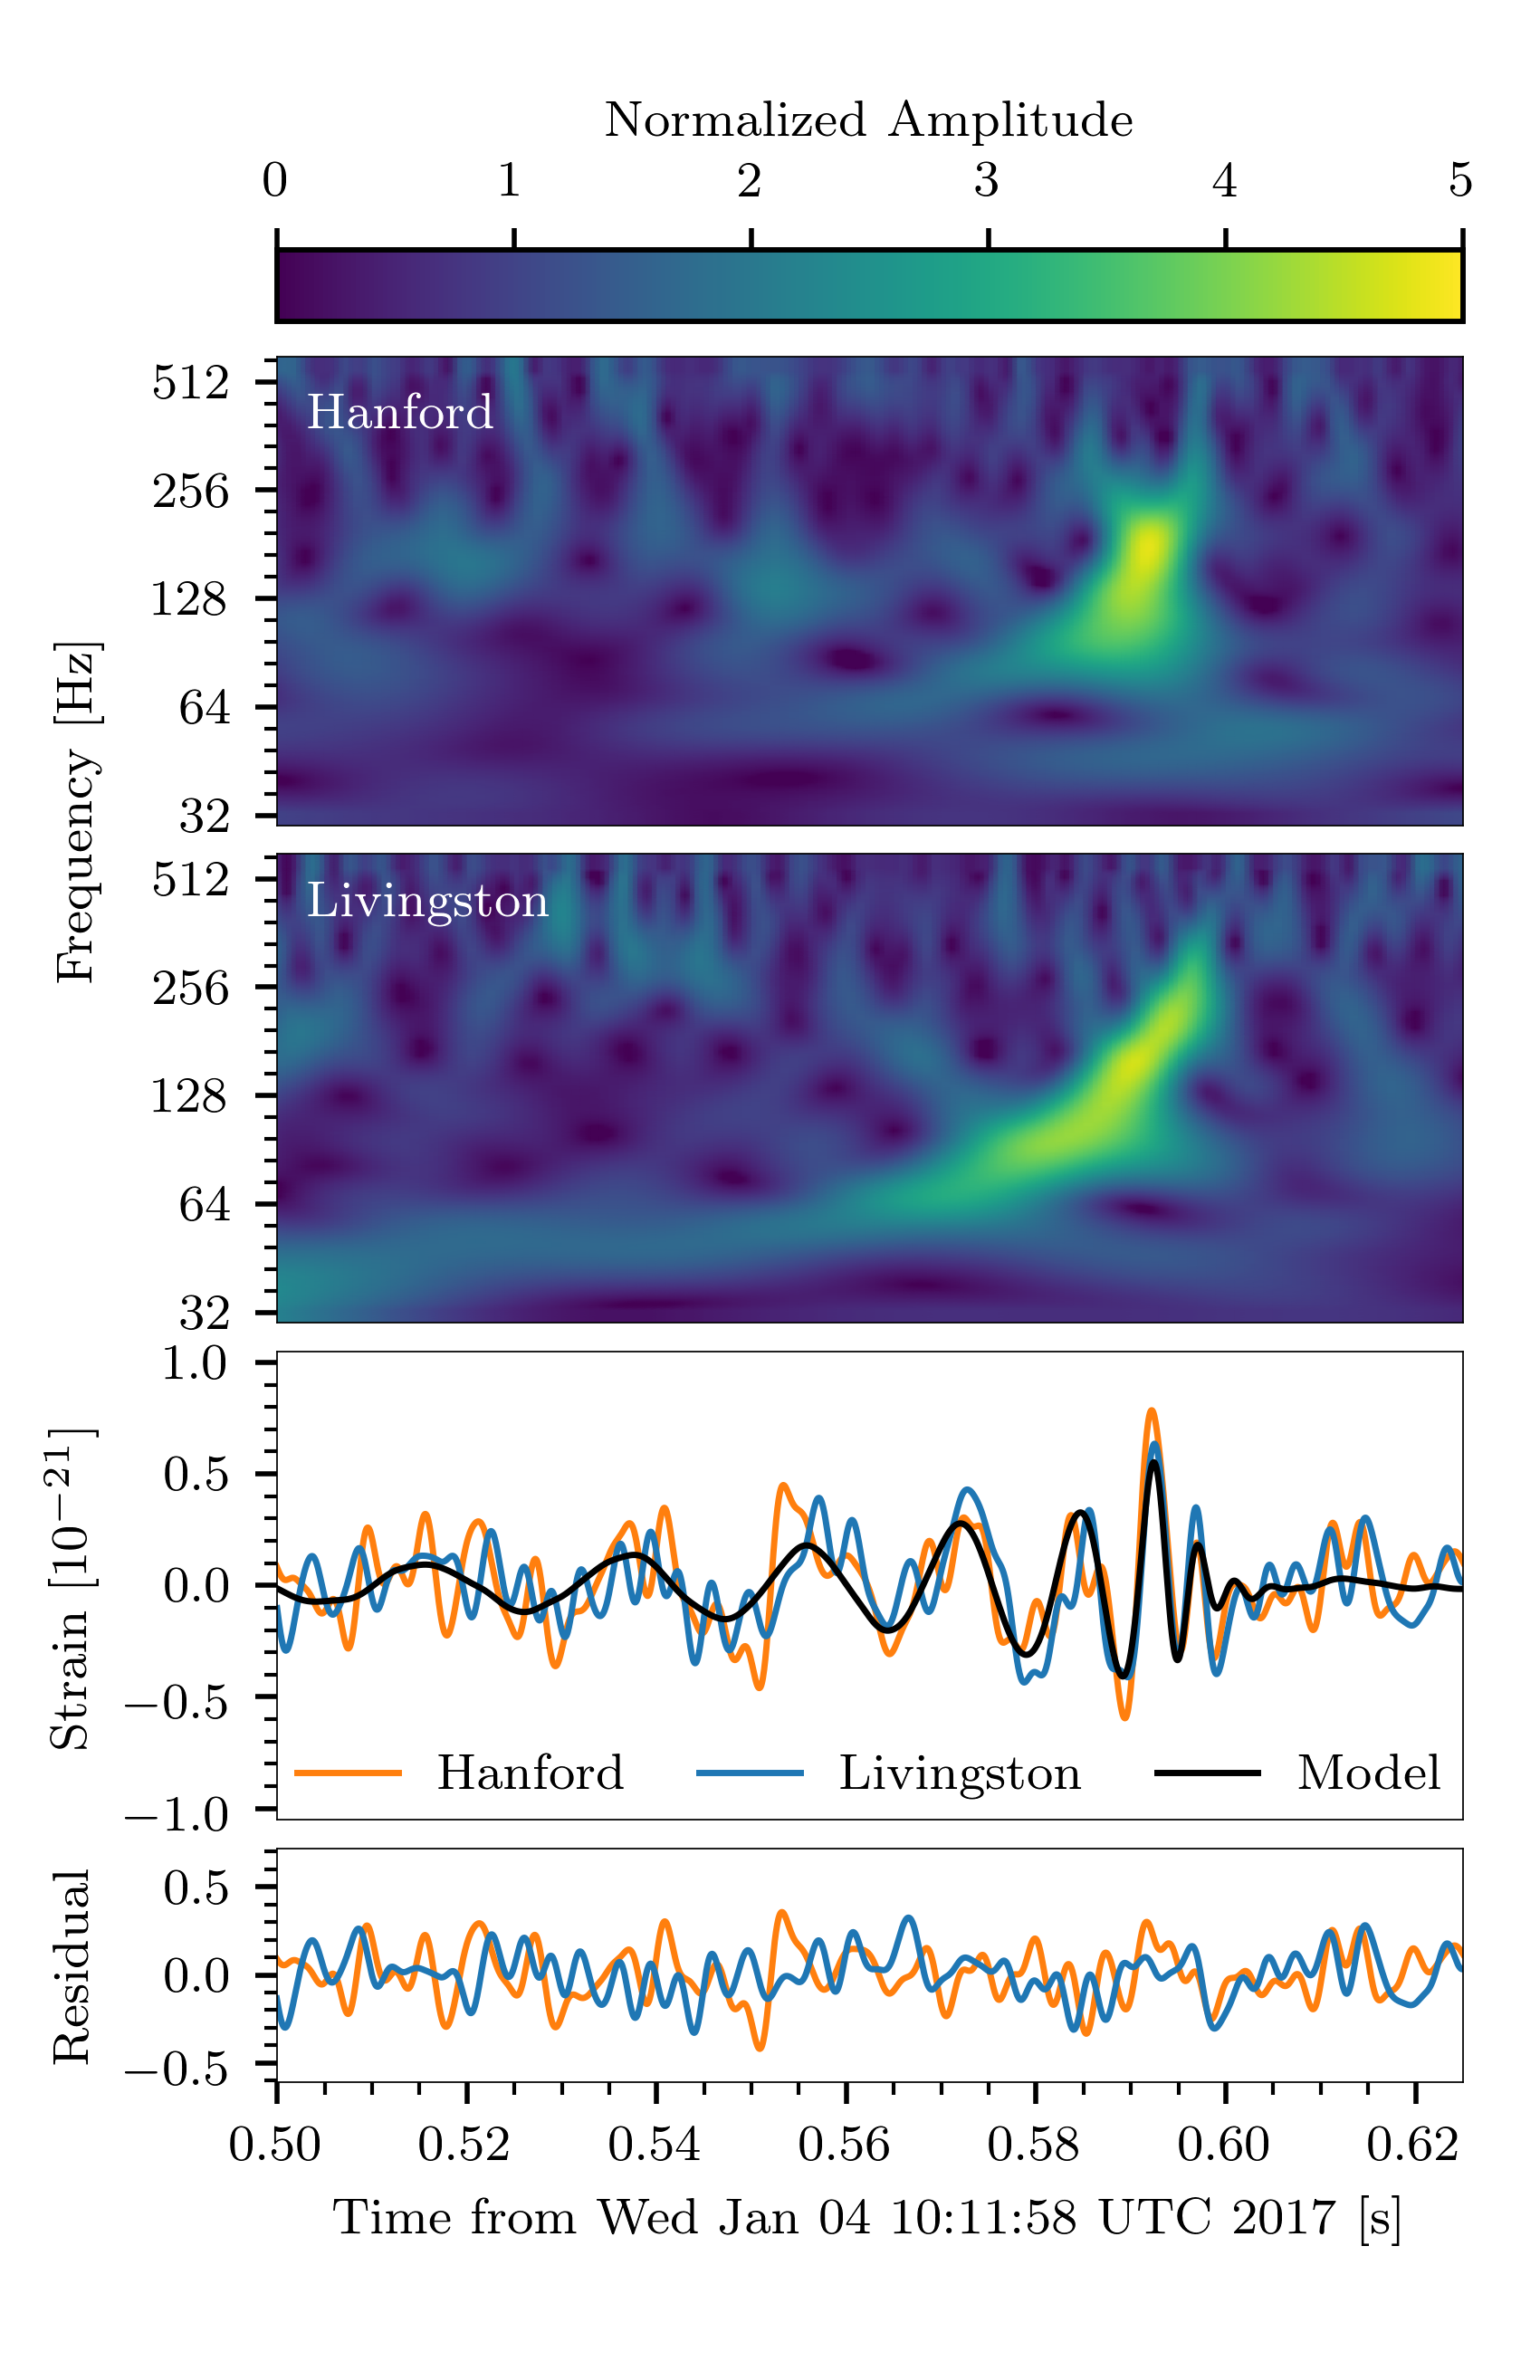
\includegraphics[scale=1.2]{images.tex/GW170104.png}
    \caption{Signal of GW170104 merger. Source :- \href{https://www.ligo.org/science/Publication-GW170104/}{LIGO.org}}
\end{figure}

Analyzing GW170104 signal yielded a new upper bound on the mass of gravitons assuming they are dispersed in vacuum like massive particles. This upper bound is equal to $7.7\times10^{-23} \, eV/c^2$. The spin axes of the black holes were unlikely to be aligned with the axis of the binary orbit. This hints that the binary black hole system was formed dynamically in a dense star cluster as an outcome of gravitational interaction between stars and binary stars, where randomly aligned spin axes are expected. The alternative scenario suggests that the system was formed out of a binary star system consisting of two main sequence stars. Although not entirely ruled out, this scenario is not favoured because black holes formed in such a binary are more likely to have positively aligned spins.

\pagebreak


\section{Advanced LIGO and other Gravitational Wave Detectors}
\input{10 Advancement}

\section{Conclusion}
\input{11 Conclusion}

\printbibliography
\end{document}
